
\documentclass[12pt]{article}
\usepackage{fullpage,enumitem,amsmath,amsthm,amsfonts,amssymb,graphicx,float,listings}

\newtheorem{thm}{Theorem}[section]
\newtheorem{cor}[thm]{Corollary}
\newtheorem{lem}[thm]{Lemma}
\newtheorem{prop}[thm]{Proposition}
\theoremstyle{definition}
\newtheorem{defn}[thm]{Definition}
\theoremstyle{remark}
\newtheorem{rem}[thm]{Remark}

% Shortcuts.
% One can define new commands to shorten frequently used
% constructions. As an example, this defines the R and Z used
% for the real and integer numbers.
%-----------------------------------------------------------------
\def\RR{\mathbb{R}}
\def\ZZ{\mathbb{Z}}

% Similarly, one can define commands that take arguments. In this
% example we define a command for the absolute value.
% -----------------------------------------------------------------
\newcommand{\abs}[1]{\left\vert#1\right\vert}

% Operators
% New operators must defined as such to have them typeset
% correctly. As an example we define the Jacobian:
% -----------------------------------------------------------------
\DeclareMathOperator{\Jac}{Jac}

%-----------------------------------------------------------------
\title{CS 221 Project Progress}
\author{Jon Braatz \& Lance Lamore}


\date{November 2018}

\begin{document}

\maketitle

\abstract{ We propose to create a model for predicting YouTube views for a video
  posted to an uploader's channel based on a candidate video title and statistics from
  previously uploaded videos to the uploader's channel. To start with, we are working with
  a dataset of composed of 6623 random video game related channels from youtube. We chose gaming videos because they are the largest category of youtbue videos that exist on the platofrom. From this list of channels, we created a simple feature vector for a video based on the channel statistics and began running a simple linear regression on the features in relation to the views of the video.}
  
\section{Previous Work}
Another team of researchers attempted a similar project that sought to
predict view counts based on an input thumbnail image and title [1]. They
performed gradient boosted regression on features from 
a dataset of YouTube videos from the Fitness \& Health category,
which they obtained from the YouTube-8M dataset that YouTube released to the
research community [2]. They also used this data to scrape information from more
videos using the YouTube API [3]. The features they used included:
a title clickbait score output from a pre-trained neural network, a ``NSFW''
score of the thumbnail image output from another pre-trained neural network,
channel subscriber count, view count, and video count, and the view count of the
channel's previous uploaded video, among other features. They found that the
most important features were features extracted from channel information and not
the features extracted from either the title or image of the video.

\section{Overview}
We sought to expand upon the previous work by shifting focus to gaming videos on Youtube.
The quantity of videos that exist on the platform demonstrate the importance to the
community. This project would be designed with content creators in mind. They would use this 
predictor as a tool to test different titles and choose the one that maximizes their viewCount. 
The premise of this project revolves around the idea of predicting the view
count of YouTube videos given features like the title
and similar information from previous videos uploaded on the same channel. We
had the initial idea of predicting views based just on a given title and
thumbnail and then using this predictor to generate video titles that are
optimized for maximizing views given a list of keywords that the title should
contain. However, previous work in this area found that the metadata of
individual videos were far less predictive of views than channel information
like subscriber count, channel view count, and channel video count. Therefore,
the input to our system will be a YouTube channel ID and a title and the 
output will be a prediction of the number of
views a video with that title and thumbnail would get if it were posted to that
channel. For example, the input ``Deep Reinforcement Learning'' and channel ID
``UCdKG2JnvPu6mY1NDXYFfN0g'' (the ID of the Stanford Engineering channel) should give an output of roughly 120000. 
  
\section{Goal and Design of the Model}


Our project is a regression task that, when given a candidate YouTube
video title and channel to upload it to, predicts the number of views a video
uploaded to the channel with that title would likely get. The statistics that
will be used to predict the view count will be the video statistics available
through the YouTube API of a subset of videos previously uploaded to the
provided channel. In particular, these statistics are:
\begin{enumerate}
  \item \texttt{ViewCount}
  \item \texttt{CommentCount}
  \item \texttt{LikeCount}
  \item \texttt{DislikeCount}
  \item \texttt{FavoriteCount}
  \end{enumerate}
The subset of videos to choose these statistics from will be the k-nearest
neighbors of the candidate video according to some similarity metric.
We chose two similarity metrics, one based on the video timestamps by considering
the statistics of the 10 most recently uploaded videos, and another based on
cosine similarity of the uploaded video titles to the candidate title.
The feature vectors are the same for both
models, and they are the video statistics of the ``most similar'' videos in the
channel to the candidate video, the model just differs in which videos those are.
We use a gradient boosted tree regressor to turn these statistics into a view
count prediction, and we use the \texttt{xgboost} machine learning library to do
so.

To train the regressor, we needed a dataset of ``candidate'' videos and
channels that they'd be uploaded to. To gather this data, we scanned through a
currently existing dataset with randomly sampled YouTube channel identifiers,
and using the YouTube search API we could pull statistics for all videos in
those channels. For our training dataset, we chose the most recently
uploaded video to each channel to act as a ``candidate'' video for that channel,
and then pulled the statistics of the 10 most similar videos to that one, both
in terms of publishing date and similarity of title according to cosine similarity.
Using the true view count of the most recently uploaded videos along with these
statistics, we could train our gradient boosted regressor.

\section{Algorithms Used}
Our problem is fundamentally a regression problem, and since we don't want to
limit ourselves to linear models, we decided to use gradient boosted regression.
We'll define a couple of terms first.

\begin{enumerate}
\item Regression: Regression consists of predicting a target value (in our case,
  the view count of a candidate video) based on several numerical or categorical
  predictors. In our case, the predictors are video statistics for the 10 videos
  in the channel that are most similar to the candidiate video according to some
  similarity metric.
\item Decision Tree: A decision tree is a method of regression that is built
  top-down from a root node and involves partitioning the data into subsets that
  contain instances with similar values. At each interior node of the tree, we
  apply a test to one of the predictor variables, and depending on the value of
  the outcome of the test we either go to the left or right subtree. Predictions
  of the target variable correspond to leaves in the tree. A decision tree
  regression algorithm will construct a decision tree based on training data
  that minimizes the least square error of the predictions and training target
  values, subject to a regularization term.

\end{enumerate}

With these two terms defined, We can go into the 6 different algorithmic approaches 
we used to solve this problem. Drawing mainly from the \texttt{sklean} library, we belived 
these methods would each provide a novel appraoche to solving this problem. 
\begin{enumerate}
    \item Ridge Regression: This is essentially an ordinary least squares regression with an added penalty for larger coefficients. Regular least square regressions assume that features are independent of each other and this can cause inaccurate predictions. This method, helps reduce the effects of collinearity in the feature space.  
    \item Lasso Regression: This is another least squares regression with a penalty factor for unimportant features. This attempts to compress the feature space and reduce the number of parameters that the out put should depend on
    \item Support Vector Machines:  Uses subset of training points in decision tree and fits it to a specified Kernel function. We chose to use to the default kernel function, the rbf function. This 
    
    \item Random Forest: This creates an ensemble of decision trees that are each trained on random sub-samples of the training set. This means a diverse set of regressions is created by introducing randomness in the regression construction. The prediction of the ensemble is given as the averaged prediction of the individual regressions.
    \item Adaptive Boosting: This is also a tree model, which uses an ensemble decision tree method that combines weak learners into a single strong one. It is trained on a modified version of the training set where the most complicated examples gain ever-increasing influence.
    \item Gradient Tree Boosting: Gradient tree boosting is based on the idea of
      creating a potentially weak regression tree on the data, creating a regression
      tree for the residuals of the first model, and then sequentially applying this
      idea to create a strong regressor out of weak regressors.
\end{enumerate}


We use gradient boosted regressors from two libraries for our project, one from
\texttt{sklearn} and the other from \texttt{xgboost}. The first library offers
an easy way to visualize the feature importances that are learned by the
regressor, and the second offers better performance when predicting new values.
Also, since our target variable, view count, ranges over many orders of
magnitude, it is better to predict the logarithm of the view count rather than
the view count itself. For this reason, by taking logarithms of the true view
counts in the training data, our loss function was effectively the mean squared
error of the logs.

\section{Results}

The Best methods all used the tree based models, meaning that Random Forest, Adaptive Boosting, and Gradient Tree boosting all provided similar results. Gradient tree boosting in general slightly outperformed the other two ensemble methods. The linear regressions and Support Vector machines performed more poorly. This is most likely because the complexity of the regression task is too nuanced, while the regression models are more simple. The table has the following performance metrics for the different methods used. $R^2$ and Mean squared error values are provided for the test set across the different predictors.  The $R^2$ values are the coefficients of determination for the prediction, where a score of 1 represents perfect prediction and a score of zero represents predicting the expected value of Y every time. $R^2$ values can be negative if the predictions are worse. 



\begin{center}
\begin{tabular}{ |c|c|c| } 
 \hline
 Algorithm Used & $R^2$ & Mean Squared Error \\ 
 \hline
 \hline
 Gradient Boosting(with NLP) & .653 & 2.231 \\ 
 \hline
 Gradient BOosting(time based) & .531 & 3.255 \\ 
 \hline
 Random Forest & .621 & 2.440\\
 \hline 
 Adaptive Boosting  & .593 & 2.618\\
 \hline
 Ridge Regression & -0.052 & 6.781 \\
 \hline
 Lasso Regression & -0.042 & 6.719 \\
 \hline
 Support Vector Regression & 0.011 & 6.368\\
 \hline
\end{tabular}
\end{center}

We see that the linear regressions models are performing extremely poorly, often doing worse than just predicting the expected value of Y. The tree models on the other hand were more far better suited for this task, provided relatively useful results. Since Gradient Boosting was the most successful predictor, we will focus on the results of this predictor for the remainder of the section. Gradient tree boosting allows for nice visualization of features weights, which are depicted below for time-based and NLP based predictors. 




\begin{figure}[H]
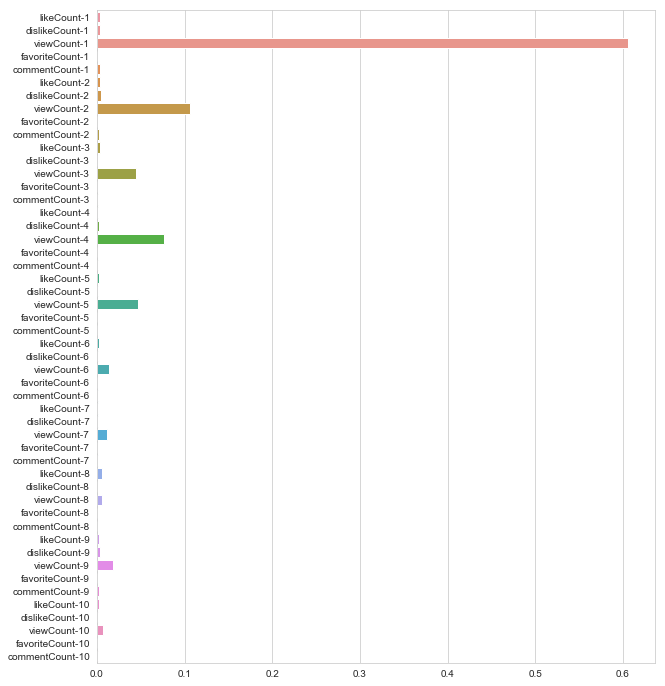
\includegraphics[width=.4\textwidth]{time_importances.png}
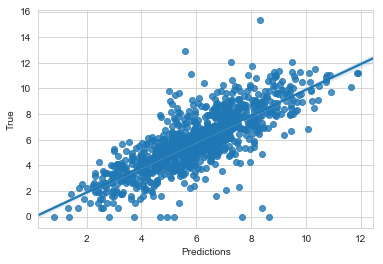
\includegraphics[width=.4\textwidth]{time_graph.png}
\caption{``The feature importances and a plot of the log-transformed viewCount
  predictions against the true viewCounts when using statistics for the 10 most
  recent videos.''}
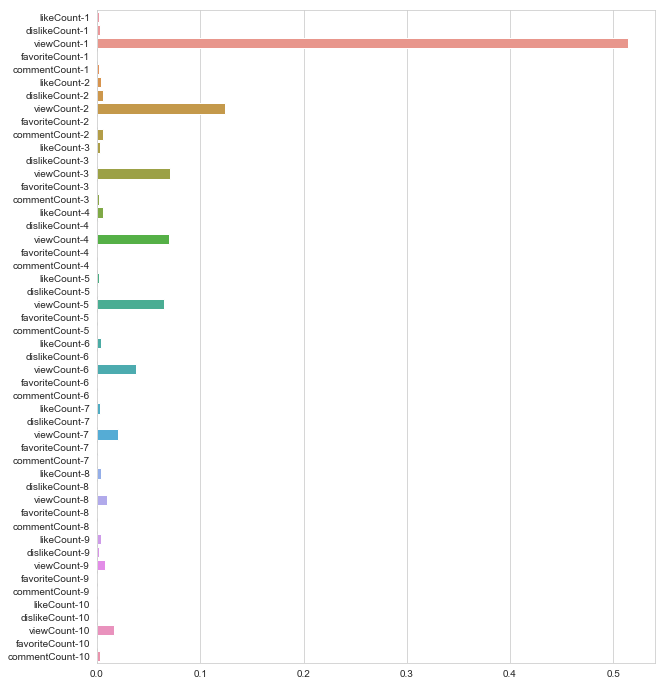
\includegraphics[width=.4\textwidth]{nlp_importances.png}
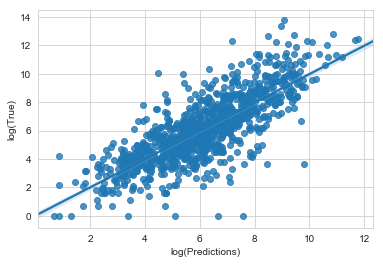
\includegraphics[width=.4\textwidth]{nlp_graph.png}
\caption{``The feature importances and a plot of the log-transformed viewCount
  predictions against the true viewCounts when using statistics for the 10 most
  similar videos according to the title's cosine similarity with the candidate title.''}
\end{figure}

We were able to beat the baseline performance when using both a video similarity
metric based on time stamp and based on cosine similarity of the title. Plotting
the feature importance's of the regression showed that the important features
match up with what one would intuitively expect. The best predictor of view
counts are the view counts of the most similar videos (either most recent or
closest in subject matter), and their predictive power drops off as the
similarity to the candidate video goes down. Other statistics besides view
counts were not found to be predictive.

On our dataset, the baseline's mean squared error between the log of the
predicted view count and the log of the true view counts in the training set was
found to be 2.2, and the oracle's was found to be .32. Our regressions based on
the statistics of most recent videos and videos with the highest cosine
similarity to the candidate title were 1.92 and 2.07 respectively, which beats
the baseline but leaves much room for improvement. The $R^2$ values for both
regressions were similar, at approximately .617 and .624 respectively.


\section{Future Work}

Moving forward, we will eliminate features that were found not to be predictive
and add more sophisticated NLP models. We can add extra features to the channel
feature vectors that come from NLP models, or we can use more sophisticated NLP
models to choose the subset of video statistics to include in the feature vector.
It's also possible that using a larger dataset would make the regression perform better.

\begin{thebibliography}{99}

\bibitem{Cd94} Aravind Srinivasan, \emph{YouTuve Views Predictor}, 

    \qquad https://towardsdatascience.com/youtube-views-predictor-9ec573090acb
\bibitem{Cd94}
YouTube 8M dataset: https://research.google.com/youtube8m/
y\bibitem{Cd94}YouTube Data API: https://developers.google.com/youtube/v3/



\end{thebibliography}

\end{document}
